\chapter{The shield}\label{cha:the-shield}

\begin{figure}[!htbp]
  \centering
  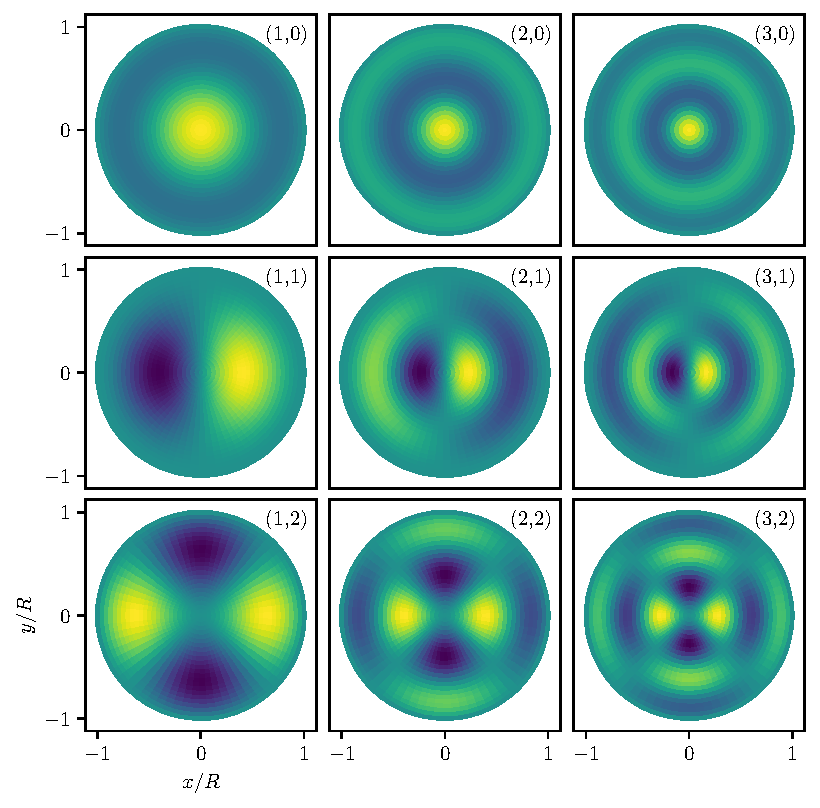
\includegraphics[width=\textwidth]{./../figures/vibrations/vibrational-modes.pdf}
  \label{fig:4:vibrational-modes}
  \caption{Vibrational modes of a spherical plate fixed at the edge with $R/d = 1000$.}
\end{figure}



Gravitational effect of the shield is neglectable
PROOF:





The modes $(k,l),\, 1 \leq k, \, 0 \leq l$ have the shape
\begin{equation}
  u_{kl}(r, \theta, t) = A\left[J_l(\sqrt{\beta_k}r) - \frac{J_l(\sqrt{\beta_k}r_s)}{I_l(\sqrt{\beta_k}r_s)}I_l(\sqrt{\beta_k}r)\right]\cos(l\theta+\phi_1)\sin(\omega_{kl}t+\phi_2)
\end{equation}
with
\begin{equation}
  \beta_k = \frac{\tilde{r}_k^2}{r_s^2} \quad \quad \omega_{kl} = \frac{\tilde{r}_k^2}{r_s^2}\sqrt{\frac{D}{\rho d}} = \tilde{x}_l^2\frac{d}{r_s^2}\sqrt{\frac{E}{12\rho(1-\nu^2)}} ,
\end{equation}
where $\tilde{r}_k$ is the $k$-th solution of the equation
\begin{equation}
  J_l(\tilde{r}_k)I_{l+1}(\tilde{r}_k)+I_l(\tilde{r}_k)J_{l+1}(\tilde{r}_k) = 0 .
\end{equation}
The amplitude A of the vibrational mode $(k,l)$ is given by $A \sim \sqrt{(\Delta z_{kl})^2_T}$ where $(\Delta z)^2 = \avg{z^2} - \avg{z}^2$ is the variance of the oscillator mode
\begin{equation}
  (\Delta z_{kl})^2_T = \frac{\hbar}{2\tilde{m}\omega_{kl}} \coth(\frac{\hbar \omega_{kl}}{2 k_B T}) .
\end{equation}
Here, $\tilde{m}$ is the effective mass of the mode which depends on the shape of the mode. It can be calculated relative to the shield mass $m=\rho \pi r_s^2 d$ by
\begin{equation}
  \tilde{m} = m\frac{1}{\pi r_s^2}\int_0^{r_s} \dd r \int_0^{2\pi} r\dd\theta \, u_{kl}(r, \theta, t) .
\end{equation}

Shield vibrations can be understood like
\begin{equation}
  \alpha = \beta = \arctan{\max_{\substack{0 \leq r \leq r_s \\ \theta \in[0, 2\pi) \\ t \in [0,2\pi/\omega_{kl})}} \abs{\pdv{r}u_{kl}(r,\theta,t)}}
\end{equation}
and
\begin{align}
  \Delta L &= u_{kl}\left(\argmax_{\substack{0 \leq r \leq r_s \\ \theta, t}} \abs{\pdv{r}u_{kl}} \right) \lesssim \sqrt{\mean{x_{kl}^2}_T} \\
  &\approx \frac{1}{r_s} \left(r_s - \argmax_{0 \leq r \leq r_s}\abs{\pdv{r}u_{kl}}\right)\sqrt{\mean{x_{kl}^2}_T}
\end{align}


\begin{figure}[!htbp]
  \centering
  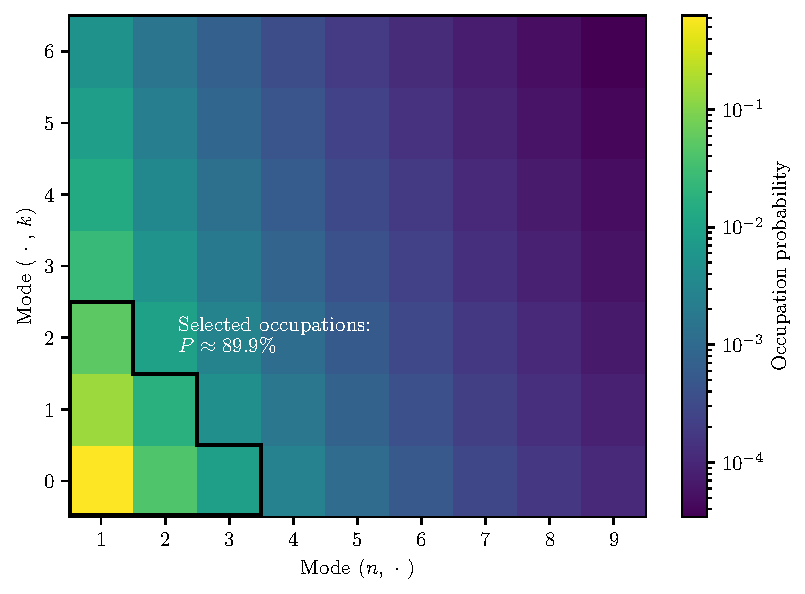
\includegraphics[width=\textwidth]{./../figures/vibrations/vibrations-mode-occupation.pdf}
  \label{fig:4:occupation-probability}
  \caption{Occupation probability of the modes at $T=4\si{K}$.}
\end{figure}